\subsection{The interaction picture} 
\textit{This section combines Prof. B. Allanach's lecture course, 
page 53 of QFT 1 Notes, University of Heidelberg, and the interaction section 
of Peskin and Schroesder}


The whole point of this section is to reduce 
solutions in our full picture, and
express them perturbatively in terms of free solutions. 
We may wish to compute a term like 
\[
\bra{ \Omega } T \phi ( x) \phi ( y ) \ket{ \Omega } 
\] where we're contracting by the ground states of the 
\textbf{full} theory, and using solutions of the full theory. Our aim is to do find out what this is in terms of free theory objects like $ \ket{ 0 } $!. 

\subsubsection{The Heisenberg and Schrodinger Picture} 
In quantum mechanics, our Schrodinger picture is when states evolve in time, and not operators. 
The obey the equation 
\[
i \frac{ d \ket{ \psi }_ s }{ d t} = H \ket{ \psi } _ s  
\] Our operators, $ \mathcal{ O } _s $, are time independent. 
On the other hand, we can also choose to be in the Heisenberg picture, 
where operators evolve instead. We define operators in the 
Heisenberg picture to obey 
\[
\mathcal{ O }_ H = e^{ i H t } \mathcal{ O  }_ s e^{  - i H t}, \quad  \ket{ \psi } _ H = e^{ i H t } \ket{ \psi }_ s  \] This ensures consistency; one can verify that 
\[
\bra{ \psi }_H \mathcal{ O } _ H \ket{ \psi } _ H =    \bra{ \psi }_S \mathcal{ O } _ H \ket{ \psi } _ S   
\] We see from the above that we can switch between our Schrodinger and Heisenberg pictures by multiplying by an appropriate time evolution factor. Heisenberg operators obey the Heisenberg equation of motion
\[
\frac{ d \mathcal{ O}^H  }{dt } = i [ H, \mathcal{ O }_H ] 
\] 

\subsubsection{The Interaction picture is a hybrid!} 
In the \textbf{interaction picture}, however, is a hybrid of the Schrodinger and Heisenberg 
picture. We separate out the free and interaction parts of the Hamiltonian as 
\[
H = H_0 + H_{ int }
\] This split is arbitrary, but we choose $ H_0 $ typically as the section which we can solve exactly. 
\begin{example}
In $ \phi ^ 4 $ theory, our Lagrangian and Hamiltonian terms associated with our interaction terms are
\[
\mathcal{ L }_{ int   }  = - \frac{\lambda}{ 4 ! }\psi ^ 4 , \quad   H_{ int }  =- \int d^ 3 x \, \mathcal{ L }_{int} = \int d^ 3 x \frac{\lambda}{4 ! } \phi^ 4 
\] Our Hamiltonian associated with the free term $ H_0 $
is given by 
\[
H_0 = \int d^ 3 x \, \frac{1}{2 } \pi ^2 + \frac{1}{2 } ( \nabla \phi) ^ 2 + \frac{1}{2 } m^ 2 \phi^ 2 
\]  
\end{example}
Our definition of our interaction picture is similar to the Heisenberg picture, exact that we are evolving states with the \textbf{free Hamiltonian}. 
This is in place of the full Hamiltonian.  
The interaction picture for a general operator is 
\[
\mathcal{ O }_ I = e^{ i H_0 t } \mathcal{ O }_s  e^{ - i H_0 t }, \implies \phi_ I ( x)  = e^{ i H_0 t } \phi_s( \vec{x} ) e^{ - H_0 t } 
\]  There's a slightly more specific way to handle this however, 
which makes use of a general reference time $ t_0 $. 
To construct the interaction picture, choose some $ t_0 $ in 
the Heisenberg picture, then evolve from $ t_0 \to t $ (philosophically, 
however, our Schrodinger picture is the same as our Heisenberg picture at 
fixed time).
\[
\phi_I( t, \vec{x} ) = e^{ i H_0 (  t- t_0 ) }\phi_H ( t_0 , \vec{x} ) e^{  - i H_0  ( t - t_0 ) }, \quad \pi_I ( t, \vec{x} ) = e^{ i H_0 ( t - t_0 ) } \pi_H ( t_0 , \vec{x} ) e^{  - i H_0 ( t -t_0 ) }
\]

\subsubsection{We can Fourier expand Interaction picture states!} 
Now, $ \phi_ I $ obeys the same commutation relations
as $ \phi $ did in the free theory: it obeys the same dynamics 
in the Heisenberg picture
\[
\dot{ \phi} _ I  = i [ H_0 , \phi_I ], \quad \dot{ \pi_I } = i [ H_0 , \pi_I]  
\] 
\begin{thm}
We have that $ \phi_ I $ also obeys the Klein-Gordon equation. 
\[
( \partial  ^ 2 + m ^ 2 ) \phi_ I ( x) = 0 
\]
\begin{proof}
Observe that for $ \phi ^ 4 $ theory, our interaction term Hamiltonian 
is a function of just $ \phi $. Thus, we have that our commutation relations remain 
exactly the same for a operators at fixed time. Thus, we have the relations for 
our conjugate momenta at fixed time, despite having an added Lagrangian
\[	
\mathcal{ L }_{\text{kinetic }}  = \frac{1}{2 } \partial _\mu \phi \partial  ^\mu \phi \implies \pi ( t_0, \vec{x} )  = \dot{\phi } ( t_0 , \vec{x} )   
\] We use this fact to our advantage in finding what 
$ \phi _ I  ( t, \vec{x} ) $  is. 
Substituting our definitions, we compute the Heisenberg equation motion 

\begin{align*}
\dot{ \phi }_I ( t_0, \vec{x} ) &=  i [ H_0 , \phi_I ( x, ) ]  \\
&=  i [ H_0 , e^{ i H_0 ( t - t_0 )  } \phi ( t_0 , \vec{x} ) e^{ - i H_0 ( t - t_0 ) }]   \\
&= i e^{ i H_0 (  t- t_0 ) } [ H_0 , \phi ( t_0, \vec{x} )  ] e^{ - i H_0 ( t - t_0 ) } \\
&= i e^{ i H_0 ( t - t_0 ) } ( - i  \pi)  ( t_0 , x ) e^{  - i H_0 ( t - t_0 ) } \\
	&=   \pi_ I ( t, x )  
\end{align*} In the above, we used the commutation relation that 
$ [ \phi ( \vec{x} ) , \pi ( \vec{y} ) ] = i \delta ( \vec{x} - \vec{y} ) $ 
to calculate $ [ H_0 , \phi ( t_0 , \vec{x} ) ] $. 
We can play exactly the same game with 
\begin{align*}
\dot{ \pi} _I ( t, x_0 ) &=  i [ H_0 , \pi_I ( t , \vec{x} ) ]  \\
&=  i e^{ i H_0 (  t- t_0 ) } [ H_0 , \pi ( t_0, \vec{x} ) ] e^{  - i H_0 ( t - t_0 ) } \\
&=  i e^{ i H_0 ( t - t_0 ) } ( - i \nabla ^ 2 \phi ( t_0 , \vec{x} ) + i m ^ 2 \phi ( t_0 , \vec{x} ) ) i e ^{  - i H_0 ( t -t_0 ) }  \\
&=  \nabla ^2 \phi_ I ( t, \vec{x} ) - m ^ 2 \phi _ I ( t, \vec{x} ) 
\end{align*}
Equating the above equation means that we deduce the Klein-Gordon equation for states in the interaction 
picture
\[
\partial _\mu \partial  ^\mu \phi_ I ( x  ) + m ^ 2 \phi_I  ( x)  =0 
\] 
\end{proof}
\end{thm} This means we could apply the exact same procedure to 
quantise this thing as we did for the free case.

\subsubsection{Operators defined from the Interaction picture obey the same commutation relations} 
Since, in the interaction picture we evolve this 
state by conjugating it either side with $ e^{ i  H_0 t }$. 
This gives us the same result that we 
has for the free field. We have that 
\[
\phi_ I ( x) = \int \frac{ d^ 3 p }{ ( 2 \pi ) ^3 } \frac{ 1 }{ \sqrt{ 2 E_p }  } (a_{ \vec{p}}  e^{  - i p \cdot  x } + a_{ \vec{p} }^\dagger e^{ i p \cdot  x } )  
\] There's an important point to be made here. 
Philosophically, these are different annihilation and 
creation operators that in our free case, so\textbf{really}, 
we should be writing, 
\[
\phi_ I ( x) = \int \frac{ d^ 3 p }{ ( 2 \pi ) ^3 } \frac{ 1 }{ \sqrt{ 2 E_p }  } (a_{ \vec{p}}^*  e^{  - i p \cdot  x } + a_{ \vec{p} }^{* \dagger}  e^{ i p \cdot  x } )  
\]
In this case, we denote $ a_{ \vec{p}}^ * , a_{\vec{p}}^ { * \dagger }  $ as 
operators which are in the \textbf{interaction} picture, 
not necessarily in the free picture. 

Despite this however, we still have that 
as before, these annihilation and 
creation operators satisfy our commutation relation as we had in 
the free theory, where 
\[
[ a_{ \vec{p} } , a_{ \vec{p}' } ^ \dagger ] = ( 2 \pi ) ^ 3 \delta ( \vec{p}- \vec{p}' ) 
\] 
A natural question to ask then is how these interaction picture
creation and operators act commute with the free-field part of the Hamiltonian, 
as well as act on the ground state. If $\phi , \pi $ are operators
associated with our full theory, and $ H_0 $ is our free Hamiltonian, 
then particular 
\begin{align*}
H_0 = e^{ i H_0 ( t - t_0) } H_0 e ^{  - iH_0 ( t - t_0) } &=   e^{ i H_0 ( t - t_0) } \left( \int d^ 3 x \, \frac{1}{2} \pi ^ 2 + \frac{1}{2 } ( \nabla  \phi ) ^ 2 + \frac{1}{2 } m ^ 2 \phi ^ 2  \right)   e ^{  - iH_0 ( t - t_0) } \\
				    &=  \int d^ 3 x \,  \frac{1}{2 } \pi_I ^ 2 +  \frac{1}{2 }( \nabla \phi_I ) ^ 2  + \frac{1}{2 } m^ 2 \phi_I ^ 2  
\end{align*}
The upshot of doing this is that we can transfer our previous analysis of raising and
lowering operators to our interaction picture. In particular, 
we have that our interaction picture annihilation and creation operators obey 
\[
[ H_0 , a_{ \vec{p} } ^ * ] = - \vec{E_p} a_{ \vec{p} }^ * , \quad [ H_0 , a_{ \vec{p} }^{ * \dagger } ] = E_{\vec{p} } a_{p } ^{ * \dagger}
\] This means that we have a state $ \ket{ 0 }  $ such that 
\[
H_0 \ket{ 0 } = 0, \quad a_{ \vec{p} }^ * \ket{ 0 } 
\] where $ H_0 $ is the \textbf{free part of our full Lagrangian}. 
Again, a philosophical point to be made is that the free part of our 
interacting Lagrangian in of the same from as just in the case of a purely free Lagrangian. 
The whole point of the interacting picture was to introduce a new state
which obeyed the Klein Gordon relation, hence having a Fourier mode expansion, 
and hence had the same commutation relations as in the free case. 

In addition, $ a_{ \vec{p} } $ annihilates the ground state of the 
free theory part in the Hamiltonian, so $ a_{ \vec{p}} \ket{ 0 }  =0 $. 

An interesting question to would be whether the physical ground state
of the free part of the full Hamiltonian is the same as if 
we were to treat the full Hamiltonian by itself. 

We have a diagram of our logical flow below 
\begin{figure}[h] 
\centering
\begin{tikzpicture}[scale =.3, node distance=3cm, align=center]
\node[rectangle] (lagr) {Get a Lagrangian $\mathcal{ L }_{\text{ free }} + \mathcal{ L }_{\text{ interaction} } $};
\node[rectangle] (congMom) [below of=lagr] {Construct $ \pi$ \\ same as free case when $\mathcal{ L }_{ \text{ interaction }}$ doesn't depend on $ \partial _\mu \phi $};  
\node[rectangle] (hamil) [below of=congMom] {Construct $ \mathcal{ H_0 }$ 'free'}; 
\node[rectangle] (kg) [right of=hamil, xshift=4cm] {Heisen. to show KG equation \\ $ \phi_I$ solves KG};
\node[rectangle] (modes) [below of=kg] {KG $ \implies $ possible  $ a_{p }, a_{p } ^ \dagger$ expansion};  
\node[rectangle] (commutation) [below of=hamil] {derive commutation relations with $ H_0 $}; 
\node[rectangle] (annihil) [below of=commutation] {annihilation and ground state $ \ket{0 } $ defined \\ $ H_0 \ket{0 } = 0, \quad a_p \ket{ 0 }  = 0 $};  
\draw[->] (lagr)--(congMom);
\draw[->] (congMom)--(hamil);
\draw[->] (hamil)--(kg); 
\draw[->] (kg) --(modes); 
\draw[->] (hamil) -- (commutation);
\draw[->] (modes) -- (commutation); 
\draw[->] (commutation) -- (annihil); 
\end{tikzpicture}
\end{figure}

\pagebreak
\subsubsection{Introducing the time unitary operator} 

Let's reparse things for the sake of generality for a bit. 
There's nothing special in our choice of $ t = 0$. 
We could have easily just fixed a time  $ t_0 $ as our reference point, 
and in our Heisenberg operator our states evolve as 
\[
\phi ( x ,t ) = e^{ i H ( t - t_0 ) } \phi ( x, t_0 ) e^{  - i H ( t - t_0 ) }
\] In the interaction picture, we set our perturbation constant $ \lambda = 0$, and thus
get the result that 
\[
\phi_I ( x, t ) = e^{ i H_0 ( t - t_0 ) } \phi( x, t_0 ) e^{ - i H_0 ( t - t_0 ) }
\] Now, how do we switch the between the two pictures? 
Well, we invert our interaction picture then multiply like so: 
\[
\phi ( x, t) = e^{ i H ( t - t_0 ) } e^{  -i H_0 ( t - t_0 ) } \phi_I ( x, t ) e^{ i H_0 ( t - t_0 ) } e^{  - i H ( t - t_0 ) }
\] Now, if we define $ U ( t, t_0 ) = e^{ i H_0 ( t - t_0 ) } e^{  - i H ( t - t_0 ) }$
The above equation simply reads as 
\[
\phi ( x, t ) = U ( t, t_0 )^{ -1 }  \phi_ I ( t , x) U ( t, t_0 ) 
\] Our operator $ U $ is a unitary time evolution operators. It has the property that 
\[
U ( t_1 , t_2) U ( t_2, t_3 ) = U ( t_1, t_3), \quad U ( t, t) = 1 
\] It also satisfies the equation that 
\begin{align*} 
i \frac{\partial  U ( t, t_0 ) }{\partial t }  &=  e^{ i H_0 ( t -t_0 ) } ( H - H_0 ) e^{  - i H ( t - t_0 ) }  \\
		       &=  e^{ i H_0 ( t - t_0 ) } H_{int} e^{  -i H ( t - t_0 ) }  \\
		       &=  e^{ i H_0 ( t - t_0 ) } H_{int} e^{  - i H_0 ( t - t_0 ) } e^{ i H_0 ( t - t_0 ) } e^{  - iH ( t - t_0 ) }\\
		       &=  H_I ( t) U ( t, t_0)  
\end{align*} In this case $ H _I ( t) $ is our interaction picture 
Hamiltonian with 
\[
H_I ( t )  = e^{ i H_0 ( t - t_0 ) } H_{ int} e^{  - i H_0 ( t - t_0 ) }
\] 
If $ H_I $ were just a function, we could solve this by setting
\[
U = \exp \left[  - i \int_{t_ 0 }^ t H_I ( t' ) dt '  \right] 
\] but this doesn't work if there are ordering ambiguities.
This is because we have that $ [ H_I ( t' ), H _I ( t'' ) ] \neq = 0 $. 
However, our differential equation for  $ U ( t, t_0 ) $ implies that it
satisfies the equation 
\[
U ( t , t_0 ) = 1 - i \int_{ t_0 }^ t dt' \, H_I ( t' ) U ( t' , t_0 ) 
\] We substitute this back into itself to  get the infinite series 
expansion 
\[
U ( t, t_0) = 1 + ( - i ) \int_{ t_0}^ t dt' H_I ( t' ) + ( -i ) ^ 2 \int_{t_0}^t dt' \int_{t_0 }^{ t' }  dt'' H_I ( t' ) H_I ( t'' ) + \dots 
\] We can already intuitively see that 
this satisfies the differential equation. 
Also, the boundary condition that $ U ( t_0 , t_0 ) $ works out. 

For the ranges of integration, the $ H_I $ product is automatically time ordered! 
We'll see why this is the case - it has to do with clever relabelling and the diagram we'll show below. 
Let's look specifically at the second order term 
\[
\int_{ t_0 } ^ t dt' \int_{ t_0 } ^{ t' } dt'' H_{ I } ( t' ) H_{ I } ( t'' ) 
\]
\begin{figure}[h]
\centering 
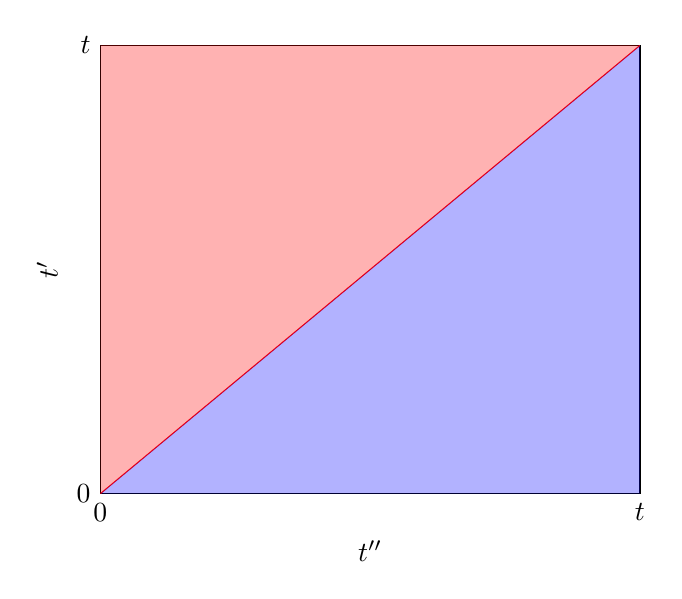
\begin{tikzpicture}
\begin{axis}[
xmin = 0, xmax = 10,
ymin = 0, ymax = 10,
xlabel=$t''$,
ylabel=$t'$,
%yticklabels=\empty,
%xticklabels=\empty,
xtick={0,10}, 
xticklabels={$0$,$t$},
ytick={0,10}, 
yticklabels={$0 $, $ t$} 
]
\addplot[red, domain=0:10] {x};


\begin{scope}
\fill [blue,opacity=.3] (0, 0) -- (100, 100) -- (100, 0);
\fill [red,opacity=.3] (0, 0) -- (100, 100) -- (0, 100); 
\end{scope}
\end{axis}

\end{tikzpicture}
\caption{The integration variables add up to a square!} 
\label{fig:intAdd}
\end{figure}

With this choice of dummy variable our integration variables
are defined so that 
\[
t \ge t' \ge  t'' > t_0 
\] This is shown in the figure \ref{fig:intAdd}. 
So, by the definition of time ordering, in this \textbf{range}, 
we have that 
\[
\int_{ t_0 } ^ t dt' \int_{ t_0 } ^{ t' } dt'' H_{ I } ( t' ) H_{ I } ( t'' ) = \int_{ t_0 } ^ t dt' \int_{ t_0 } ^{ t' } dt'' \mathcal{ T } ( H_{ I } ( t' ) H_{ I } ( t'' ) ) \] However, integration variables are just dummies, so 
we can relabel them. If we relabel $ t' \to t''$, and 
$ t'' \to  t' $, then we have that 
\[
\int_{ t_0 } ^ t dt'' \int_{ t_0 } ^{ t'' } dt' H_{ I } ( t'' ) H_{ I } ( t' )  = \int_{ t_0 } ^ t dt' \int_{ t_0 } ^{ t' } dt'' H_{ I } ( t' ) H_{ I } ( t'' ) 
\] But in this case, our first expression has ranges defined by $ t \geq t'' \geq t' > t_0 $. 
This is the red portion of our square in 
the diagram. 
This is also consistent with time ordering, so we can put our time ordering symbol in the integrand 
so that in this range, $ H_{ I } (t'') H_{ I  }  ( t' ) = \mathcal{ T } ( H _I ( t' ) H _ I ( t'' ) ) $.  
Hence, we can write our second term as 

\[
\int_{ t_0 } ^ t dt' \int_{ t_0 } ^{ t' } dt'' H_{ I } ( t' ) H_{ I } ( t'' ) =\frac{1}{2 } \left(  \int_{ t_ 0 } ^ t dt'' \int_{ t_0 }^{ t''} dt' \mathcal{ T } ( H_{ I }( t' ) H_{ I } ( t'' )  + \int _{ t_0 } ^ t dt' \int_{ t_0  }^{ t' } dt'' \mathcal{ T } ( H_I ( t' ) H _ I ( t'' ) ) \right)  
\] So, we have the same term in the integrand, $ \mathcal{ T } ( H_ I ( t' ) H _ I ( t'') $!
But, the ranges combined on the right hand side of 
this expression is just the full square. 
Hence, we can just integrate over the whole square to get that that
\[
\int_{ t_0 } ^ t dt' \int_{ t_0 } ^{ t' } dt'' H_{ I } ( t' ) H_{ I } ( t'' ) = \frac{1}{2 } \int_{ t_0 } ^ t dt' \int_{ t_0  }^ t dt'' \mathcal{ T } ( H _I ( t' ) H_ I ( t'' ) )  
\]  In full generality, we can expand this 
idea to more integrals and write 
\[
\int_{ t_0  } ^ t dt_1 \int_{ t_ 0 } ^{ t_1 } dt_2 \dots \int_{ t_0 } ^{ t_{ n - 1  } } dt_{ n } H_I ( t_1) \dots  H_{ I } ( t_{ n } )  = \frac{1}{n ! } \int_{ t_0 } ^ t dt_1 \dots \int_{ t_0 } ^{ t  } \mathcal{ T } \left(  H _ I ( t_1 ) \dots H _ I ( t_{ n } )  \right) 
\]  
Thus, we can write 
\[
U ( t, t_0) = 1 + ( -i ) \int_{ t_0 } ^ t dt' H_I ( t' ) + \frac{ ( -i ) ^ 2 }{2 } \int_{ t_0 }^t dt' \int_{ t_0 }^ t dt'' T \left\{  H_I ( t' ) H_I ( t'' )  \right\}  
\] This is Dyson's formula. 
\[
U ( t, t_0) = T \text{ exp } \left\{  - i \int_{ t_0 } ^ t dt' \, H_I ( t' )  \right\} 
\] Alternatively was have that, using the Lagrangian instead, that 
\[
U ( t, t_0 ) = T \exp \left\{  i \int_{ t_0 } ^ t  d^ 3 x dt ' \mathcal{ L }_ I ( t' )  \right\} 
\] For scalar Yukawa theory,  this would be 
\[
T \exp \left\{   - i g \int d^  4 x \psi ^ * \psi \phi  \right\} 
\] This is something of a formal result. 
We expand this to finite order to get some results for scattering
amplitudes which we will derive below in the next section. 

